\documentclass[serif, aspectratio=169]{beamer}
%\documentclass[serif]{beamer}  % for 4:3 ratio

\usepackage[T1]{fontenc} 
\usepackage[utf8]{inputenc}
\usepackage{fourier} % see "http://faq.ktug.org/wiki/uploads/MathFonts.pdf" for other options
\usepackage{hyperref}
\usepackage{latexsym,amsmath,xcolor,multicol,booktabs,calligra}
\usepackage{graphicx,pstricks,listings,stackengine}
\usepackage{lipsum}
\usepackage{../HKUSTstyle}

%imports customs%
\usepackage{caption}    % for subfigures
\usepackage{subcaption} % for subfigures
\usepackage{ragged2e}
\usepackage{booktabs,makecell}
\usepackage{colortbl}
\usepackage{multirow}
\usepackage{cite}
\usepackage{tcolorbox}
\usepackage[sort,authoryear]{natbib}

\author{Julien Bezançon}

\title{Découverte du Traitement Automatique des Langues}
\subtitle{Hors-série 1~: Les expressions régulières}

\institute{julien.bezancon@univ-lorraine.fr / \url{https://julienbez.github.io}}

\date{}

% defs
\def\cmd#1{\texttt{\color{red}\footnotesize $\backslash$#1}}
\def\env#1{\texttt{\color{blue}\footnotesize #1}}

% set colors
\definecolor{hkustyellow}{RGB}{167, 131, 55}
\definecolor{hkustblue}{RGB}{0, 56, 116}
\definecolor{hkustred}{RGB}{209, 51, 59}

\lstset{
    basicstyle=\ttfamily\small,
    keywordstyle=\bfseries\color{deepblue},
    emphstyle=\ttfamily\color{deepred},    % Custom highlighting style
    stringstyle=\color{deepgreen},
    numbers=left,
    numberstyle=\small\color{halfgray},
    rulesepcolor=\color{red!20!green!20!blue!20},
    frame=shadowbox,
}

\begin{document} %  --- --- --- --- --- --- --- --- --- --- --- --- 

\begin{frame}[noframenumbering,plain]
    \titlepage
    \vspace*{-0.6cm}
    \begin{figure}[htpb]
        \begin{center}
            \hspace{0.3cm}
            
\includegraphics[width=0.7\columnwidth]{../../../IMAGES/loria_idmc.png}
        \end{center}
    \end{figure}
\end{frame}

% \begin{frame}    
%     \tableofcontents[sectionstyle=show,
%     subsectionstyle=show/shaded/hide,
%     subsubsectionstyle=show/shaded/hide]
% \end{frame}

\section{Avant de commencer...}

\begin{exoframe}{}
    \begin{center}
        \Large
        De quoi avons-nous discuté lors du derniers cours ? \\
        Avez-vous des questions ?
    \end{center}
\end{exoframe}

\begin{frame}{Références de ce cours}
    \begin{itemize}
        \item Gaël Lejeune (gael.lejeune@sorbonne-universite.fr)
        \begin{itemize}
            \item cours d'ingénierie des langues
        \end{itemize}
        \vspace{10pt}
        \item Maxime Amblard (maxime.amblard@univ-lorraine.fr)
        \begin{itemize}
            \item cours de découverte du TAL
        \end{itemize}
        % \vspace{10pt}
        % \item Julien Romero (julien.romero@telecom-sudparis.eu)
        % \begin{itemize}
        %     \item cours d'introduction au TAL
        % \end{itemize}
    \end{itemize}
\end{frame}


% \begin{frame}{Un peu de contexte}
%     % \begin{block}{Traitement de texte en TAL}
%     %     \begin{itemize}
%     %         \item Segmentation
%     %         \item Tokenisation
%     %         \item Lemmatisation (ou racinisation)
%     %         \item Étiquetage morphosyntaxique
%     %     \end{itemize}
%     % \end{block}
%     \begin{center}
%         \Large
%         Parfois, on a besoin d'accéder rapidement à l'information. \\
%         Les techniques du TAL prennent du temps à mettre en place.
%     \end{center}
%     \vspace{10pt}
%     \begin{block}{Exemple~: identifier...}
%         \begin{itemize}
%             \item des adresses mails
%             \item des numéros de téléphone
%             \item les mots se terminant par -able
%             \item des formats d'image (.png, .svg, etc)
%         \end{itemize}
%     \end{block}
% \end{frame}

\section{Les expressions régulières}

\begin{frame}{Un petit test}
    \begin{block}{Identifiez tous les noms et prénoms dans ce texte\footnote{Le Seigneur des anneaux, Tome 1 : La Communauté de l'Anneau de J. R. R. Tolkien}}
        \justify
         << Le travail était principalement effectué par son plus jeune fils, Sam Gamegie. Tant le père que le fils étaient en relations très amicales avec Bilbon et Frodon. Ils habitaient sur la Colline même, au numéro 3 du Chemin des Trous-du-Talus, juste sous Cul-de-Sac. >>
    \end{block}
    \vfill
    \pause
    \begin{block}{Deux manières pour rechercher des informations}
        \begin{itemize}
            \item Recherche en extension~: lister toutes les formes attendues
            \begin{itemize}
                \item Sam, Gamegie, Bilbon, Frodon
            \end{itemize}
            \item Recherche en intension~: définir des règles pour identifier les formes attendues
            \begin{itemize}
                \item Commence par une majuscule
            \end{itemize}
        \end{itemize}
    \end{block}
\end{frame}

\begin{frame}{Les expressions régulières}
    \begin{block}{Définition de Wikipédia\footnote{\url{https://fr.wikipedia.org/wiki/Expression_régulière}}}
        \begin{tcolorbox}
            En informatique, une expression régulière est une chaîne de caractères qui décrit, selon une syntaxe précise, un ensemble de chaînes de caractères possibles. Les expressions régulières sont également appelées \textbf{regex}.
        \end{tcolorbox}
    \end{block}
    \begin{center}
        \Large
        Les regex permettent d'identifier des motifs dans des textes. \\
        Motif~: structure formelle et régulière.
    \end{center}
\end{frame}

\begin{frame}{Qu'appelle-t-on un motif ?}
    \begin{block}{Motifs institutionnalisés}
        \begin{itemize}
            \item Urls
            \item Adresses mails
            \item Numéros de téléphone
            \item Formats d'image (.png, .svg, etc)
        \end{itemize}
    \end{block}
    \begin{block}{Motifs langagiers}
        \begin{itemize}
            \item Exemple~: trouver les expressions de la forme "prendre la X"
            \item Ce qu'on cherche~: prendre la parole, prendre la porte, etc 
        \end{itemize}
    \end{block}
    \begin{center}
        \Large
        Une regex permet de prendre en compte toutes \\ 
        les variantes possibles d'un motif.
    \end{center}
\end{frame}

\begin{exoframe}{Exercice}
    \begin{block}{Identifiez le motif de...}
        \begin{itemize} \color{white}
            \item Tous les numéros de téléphone français
            \item Toutes les adresses mails
        \end{itemize}
    \end{block}
    \vspace{15pt}
    \begin{center}
        \Large
        Utilisez vos mots pour décrire ces motifs !
    \end{center}
\end{exoframe}

\begin{frame}{Solutions possibles}
    \begin{block}{Numéros de téléphone}
        \begin{itemize}
            \item 8 nombres, les deux premiers sont listables (01, 03, 06, 07, etc)
            \item Et pour ces numéros ? $\Rightarrow$ 01 01 23 45 67 || 01-01-23-45-67
        \end{itemize}
    \end{block}
    \begin{block}{Adresses mails}
        \begin{itemize}
            \item une séquence + @ + une séquence + un suffixe (.com, .fr, etc)
            \item bezanconjulien@gmail.com || julien.bezancon@univ-lorraine.fr
            %\item bezancon@lisn.fr
        \end{itemize}
    \end{block}
    \begin{block}{Avec des regex} %TODO : les améliorer
        \begin{itemize}
            \item Numéros~: ((\bs +33)|0)\bs d{9}
            \item Mails~: \nothing [\bs w\bs -\bs .]+@([\bs w-]+\bs .)+[\bs w-]\{2,4\}
        \end{itemize}
    \end{block}
\end{frame}

\begin{frame}{Quelques règles}
    \begin{block}{Chaque caractère se reconnait lui-même (majuscules et espaces compris)}
        \begin{itemize}
            %\item les majuscules et les espaces comptent
            \item "lapin" reconnait "lapin", mais pas "Lapin"
            \item "France 2" ne reconnait pas "France 3" ou "France2"
        \end{itemize}
    \end{block}
    \begin{block}{Des métacaractères existent}
        \begin{itemize}
            \item Les opérateurs %$\Rightarrow$ fournissent des instructions complexes
            \item les quantifieurs %$\Rightarrow$ indiquent le nombre de répétitions d'un caractère
        \end{itemize}
    \end{block}
    \begin{center}
        \Large
        Motif~: mélange de caractères et métacaractères. \\
        France \bs d $\Rightarrow$ reconnait "France 2", "France 3", etc
    \end{center}
\end{frame}

\section{Syntaxe d'une regex}

\begin{frame}{Opérateurs}
    \begin{table}
        \renewcommand{\arraystretch}{1.5}  
        \raggedright
        \begin{tabular}{|c|p{10cm}|}
            \hline
            () & groupe de caractères \\
            \hline
            . & n'importe quel caractère \\
            \hline
            | & une expression OU une autre expression \\
            \hline
            $\hat{}$ & condition~: expression au début de ligne \\
            \hline 
            \$ & condition~: expression en fin de ligne \\
            \hline
            {[} {]} & n'importe quel caractère entre les crochets \\
            \hline
            {[} $\hat{}$ {]} & n'importe quel caractère qui n'est pas entre les crochets \\
            \hline
        \end{tabular}
    \end{table}
\end{frame}

\begin{frame}{Quantifieurs}
    \begin{table}
        \renewcommand{\arraystretch}{1.5}  
        \raggedright
        \begin{tabular}{|c|p{9.5cm}|}
            \hline
            ? & une expression 0 ou 1 fois \\
            \hline
            + & une expression 1 fois ou plus \\
            \hline
            * & une expression 0 fois ou plus \\
            \hline
            \{n\} & une expression exactement n fois \\
            \hline
            \{n,m\} & une expression entre n et m fois \\
            \hline
            \{n,\} & une expression au moins n fois \\
            \hline
            \{,m\} & une expression au plus m fois \\
            \hline
        \end{tabular}
    \end{table}
\end{frame}

\begin{frame}{Classes de caractères}
    \begin{table}
        \renewcommand{\arraystretch}{1.5}  
        \raggedright
        \begin{tabular}{|c|p{9.8cm}|}
            \hline
            \bs w & caractères alphanumériques \\
            \hline
            \bs W & caractères autres que alphanumériques \\
            \hline
            \bs s & caractères d'espacement \\
            \hline
            \bs S & caractères autres que ceux 
            d'espacement \\
            \hline
            \bs d & chiffres décimaux \\
            \hline
            \bs D & caractères autres que chiffres décimaux \\
            \hline
        \end{tabular}
    \end{table}
\end{frame}

\begin{exoframe}{Exercices}
    \begin{block}{Quelles expressions les regex suivantes peuvent-elles identifier ?}
        \begin{itemize} \color{white}
            \item lo+ng, (long)?, (lo)*ng
            \item madame|monsieur, (madame)|(monsieur)
            \item ver[ts], ver((re)|(ts)|(tige))
            \item chaton\{1,3\}, (chaton)\{1,3\}, chaton\{1,\}
        \end{itemize}
    \end{block}
    \begin{block}{Trouvez une regex pour exprimer chaque ensemble proposé}
        \begin{itemize} \color{white}
            \item Ensemble 1~: 1742479298, 987654321 , 6754, 42
            \item Ensemble 2~: aaaa, bbbb, cccc, dddd, eeeee
            \item Ensemble 3~: les conjugaisons de "aller" au présent
            \item Ensemble 4~: tous les nombres décimaux
        \end{itemize}
    \end{block}
\end{exoframe}

\begin{frame}{Trucs et astuces}
    \begin{block}{"\bs " permet de dé-spécialiser des caractères}
        \begin{itemize}
            \item \bs . $\Rightarrow$ un simple point
            \item \bs ( $\Rightarrow$ une simple parenthèse
        \end{itemize}
    \end{block}
    \begin{block}{"{[} {]}" peut s'utiliser d'une autre manière}
        \begin{itemize}
            \item {[}a-z{]} $\Rightarrow$ toutes les lettres de "a" à "z"
            \item {[}A-Z{]} $\Rightarrow$ toutes les lettres de "A" à "Z"
            \item {[}1-9{]} $\Rightarrow$ tous les chiffres de "1" à "9"
        \end{itemize}
    \end{block}
\end{frame}

\begin{exoframe}{Un exercice Rock'n'Roll (1/2)}
    \begin{center}
        \Large 
        Allez sur le site suivant~: \url{https://regex101.com/} \\
        Sinon, sortez vos crayons !
    \end{center}
    \begin{figure}
        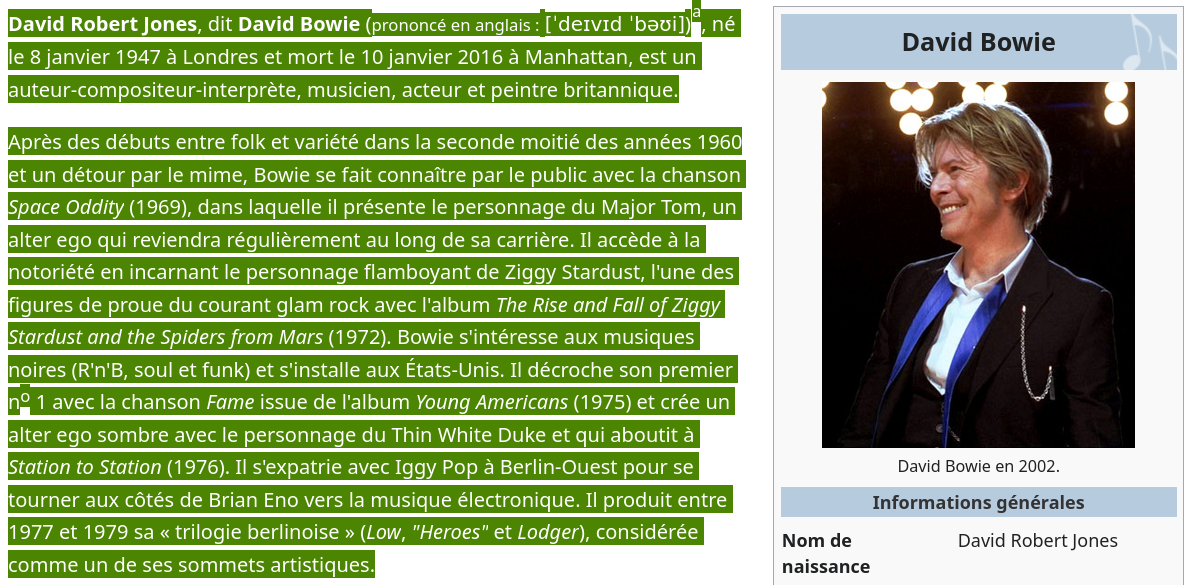
\includegraphics[width=0.7\columnwidth]{../../../FIGURES/découverte_tal/regex_bowie.png}
    \end{figure}
\end{exoframe}

\begin{exoframe}{Un exercice Rock'n'Roll (2/2)}
    \begin{block}{Créez des regex afin de pouvoir identifier...}
        \begin{itemize} \color{white}
            \item tous les mots \only<2->{$\Rightarrow$ \bs w+}
            \item toutes les années \only<2->{$\Rightarrow$ \bs d\{4\}}
            \item toutes les phrases \only<2->{$\Rightarrow$ \bs s+|[~$\hat{}$~.~!~?]*[.~!~?]}
            \item les dates complètes \only<2->{$\Rightarrow$ \bs d\{1,2\} \bs w* \bs d\{4\}}
            \item "David" ou "Bowie" + le mot suivant \only<2->{$\Rightarrow$ (David)|(Bowie) ((\bs w)|([~$\hat{}$ \bs w\bs s]))*}
        \end{itemize}
    \end{block}
\end{exoframe}

\begin{frame}{Limites}
    \begin{block}{Reprenons le dernier exercice}
        \begin{itemize}
            \item Identifiez tous les noms et prénoms
            \item Identifiez les séquences sujet/verbe/complément
            \item Identifiez les noms d'album de David Bowie
        \end{itemize}
    \end{block}
    \begin{center}
        \Large
        Les regex ne peuvent pas tout faire. \\
        Elles peuvent devenir dures à lire et comprendre. \\
        \vspace{10pt}
        $\hat{}$([a-z0-9\_\bs .-]+)@([\bs da-z\bs .-]+)\bs .([a-z\bs .]\{2,6\})\$
    \end{center}
\end{frame}

\begin{frame}{Pour résumer}
    \begin{block}{Les regex permettent de...}
        \begin{itemize}
            \item Retrouver des informations dans un texte
            \item Exprimer diverses expressions à l'aide d'un unique motif
            \item Procéder des textes afin de les traiter en TAL
        \end{itemize}
    \end{block}
    \vspace{15pt}
    \begin{center}
        \Large
        Prochain cours~: on reprend le cours de la dernière fois !
    \end{center}
\end{frame}

% slide pk on ne fait pas tout en regex : identifier les noms de famille : Un magicien n'est jamais en retard, Frodon Sacquet, ni en avance d'ailleurs. Il arrive précisément à l'heure prévue. => comment distinguer frodon de saquet ?

\end{document}
